\chapter{Utilisation de \emph{Qiskit}}\label{ch:qiskit}

Toutes les expériences présentées dans ce manuscrit ont été réalisées à l'aide de \emph{Qiskit}.
C'est un module Python développé par IBM permettant de manipuler des circuits quantiques et de les simuler.
Il permet également de les envoyer sur des ordinateurs quantiques réels fournis par IBM, ainsi que sur des
simulateurs plus performants que ceux fournis par défaut.\\
Sur le site se trouvent de nombreux tutoriels et exemples d'utilisation, ainsi que la documentation complète
du module.
De plus, l'accès aux ordinateurs quantiques est gratuit, il suffit de créer un compte sur le site, qui offre
également des serveurs Jupyter pour faire tourner les notebooks, et des outils pour visualiser les circuits
quantiques.\\ \\
Dans cette annexe, nous allons présenter le script utilisé pour construire les circuits quantiques
de certains chapitres, et les fonctions utilisées pour les simuler et les envoyer sur des ordinateurs
quantiques réels.\\
Pour cela, nous allons faire la démonstration avec les scripts utilisés pour l'algorithme de Shor,
qui ont l'avantage de couvrir de nombreux aspects du module.
De plus, la structuration étant en grande partie tirée de la documentation de \emph{Qiskit}, il est d'autant
plus facile de s'y retrouver.\\ \\
Dans un premier temps, nous allons importer les modules nécessaires à la construction du circuit quantique,
ainsi qu'à sa visualisation et à sa simulation.
De plus, les modules standards du traitement de données sont importés, ainsi que les fonctions mathématiques
afin de pouvoir traiter les résultats et faire des calculs dans le script.\\
Dans cette étape d'initialisation, nous allons également définir la manière dont nous allons simuler le
circuit quantique de manière générale sur le script, dans ce cas le simulateur \emph{qasm\_simulator}
qui est une méthode de simulation tournant localement sur l'ordinateur.\\

\begin{pyin}
import matplotlib.pyplot as plt
import numpy as np
from qiskit import *
from qiskit.visualization import plot_histogram
from math import gcd
from numpy.random import randint
import pandas as pd
from fractions import Fraction

from qiskit.visualization import plot_histogram
from qiskit.circuit.library import QFT

import math

sim = Aer.get_backend('qasm_simulator')
\end{pyin}

Dans les cellules suivantes sont définies les fonctions qui vont être utilisées pour construire le circuit,
comme l'exponentiation modulaire, la transformée de Fourier quantique inverse, ou encore les valeurs de $a$ à tester
et de qubits de comptage.\\

\begin{pyin}
def c_amod15(a, power):
    """Controlled multiplication by a mod 15"""
    if a not in [2,4,7,8,11,13]:
        raise ValueError("'a' must be 2,4,7,8,11 or 13")
    U = QuantumCircuit(4)
    for _iteration in range(power):
        if a in [2,13]:
            U.swap(2,3)
            U.swap(1,2)
            U.swap(0,1)
        if a in [7,8]:
            U.swap(0,1)
            U.swap(1,2)
            U.swap(2,3)
        if a in [4, 11]:
            U.swap(1,3)
            U.swap(0,2)
        if a in [7,11,13]:
            for q in range(4):
                U.x(q)
    U = U.to_gate()
    U.name = f"{a}^{power} mod 15"
    c_U = U.control()
    return c_U
\end{pyin}

\begin{pyin}
N_COUNT = 8  # number of counting qubits
a = 7
# Specify variables
\end{pyin}

\begin{pyin}
def qft_dagger(n):
    """n-qubit QFTdagger the first n qubits in circ"""
    qc = QuantumCircuit(n)
    # Don't forget the Swaps!
    for qubit in range(n//2):
        qc.swap(qubit, n-qubit-1)
    for j in range(n):
        for m in range(j):
            qc.cp(-np.pi/float(2**(j-m)), m, j)
        qc.h(j)
    qc.name = "QFT+"
    return qc
\end{pyin}

Dans la cellule suivante, nous allons construire le circuit quantique.
Nous commençons par créer les registres quantiques et classiques, puis nous initialisons le circuit quantique.
Ensuite, nous appliquons les portes désirées pour le circuit, et finalement, nous le dessinons afin de
pouvoir le visualiser.\\

\begin{pyin}
qr = QuantumRegister(N_COUNT + 4)
cr = ClassicalRegister(N_COUNT)
qc = QuantumCircuit(qr, cr)
# Create QuantumCircuit with N_COUNT counting qubits
# plus 4 qubits for U to act on

# Initialize counting qubits
# in state |+>
for q in range(N_COUNT):
    qc.h(q)

# And auxiliary register in state |1>
qc.x(N_COUNT)

# Do controlled-U operations
for q in range(N_COUNT):
    qc.append(c_amod15(a, 2**q),
              [q] + [i+N_COUNT for i in range(4)])

# Do inverse-QFT
qc.append(qft_dagger(N_COUNT), range(N_COUNT))

# Measure circuit
qc.measure(range(N_COUNT), range(N_COUNT))
qc.draw(fold=-1, output='mpl')  # -1 means 'do not fold'
\end{pyin}

\begin{pyout}
;@ \begin{center}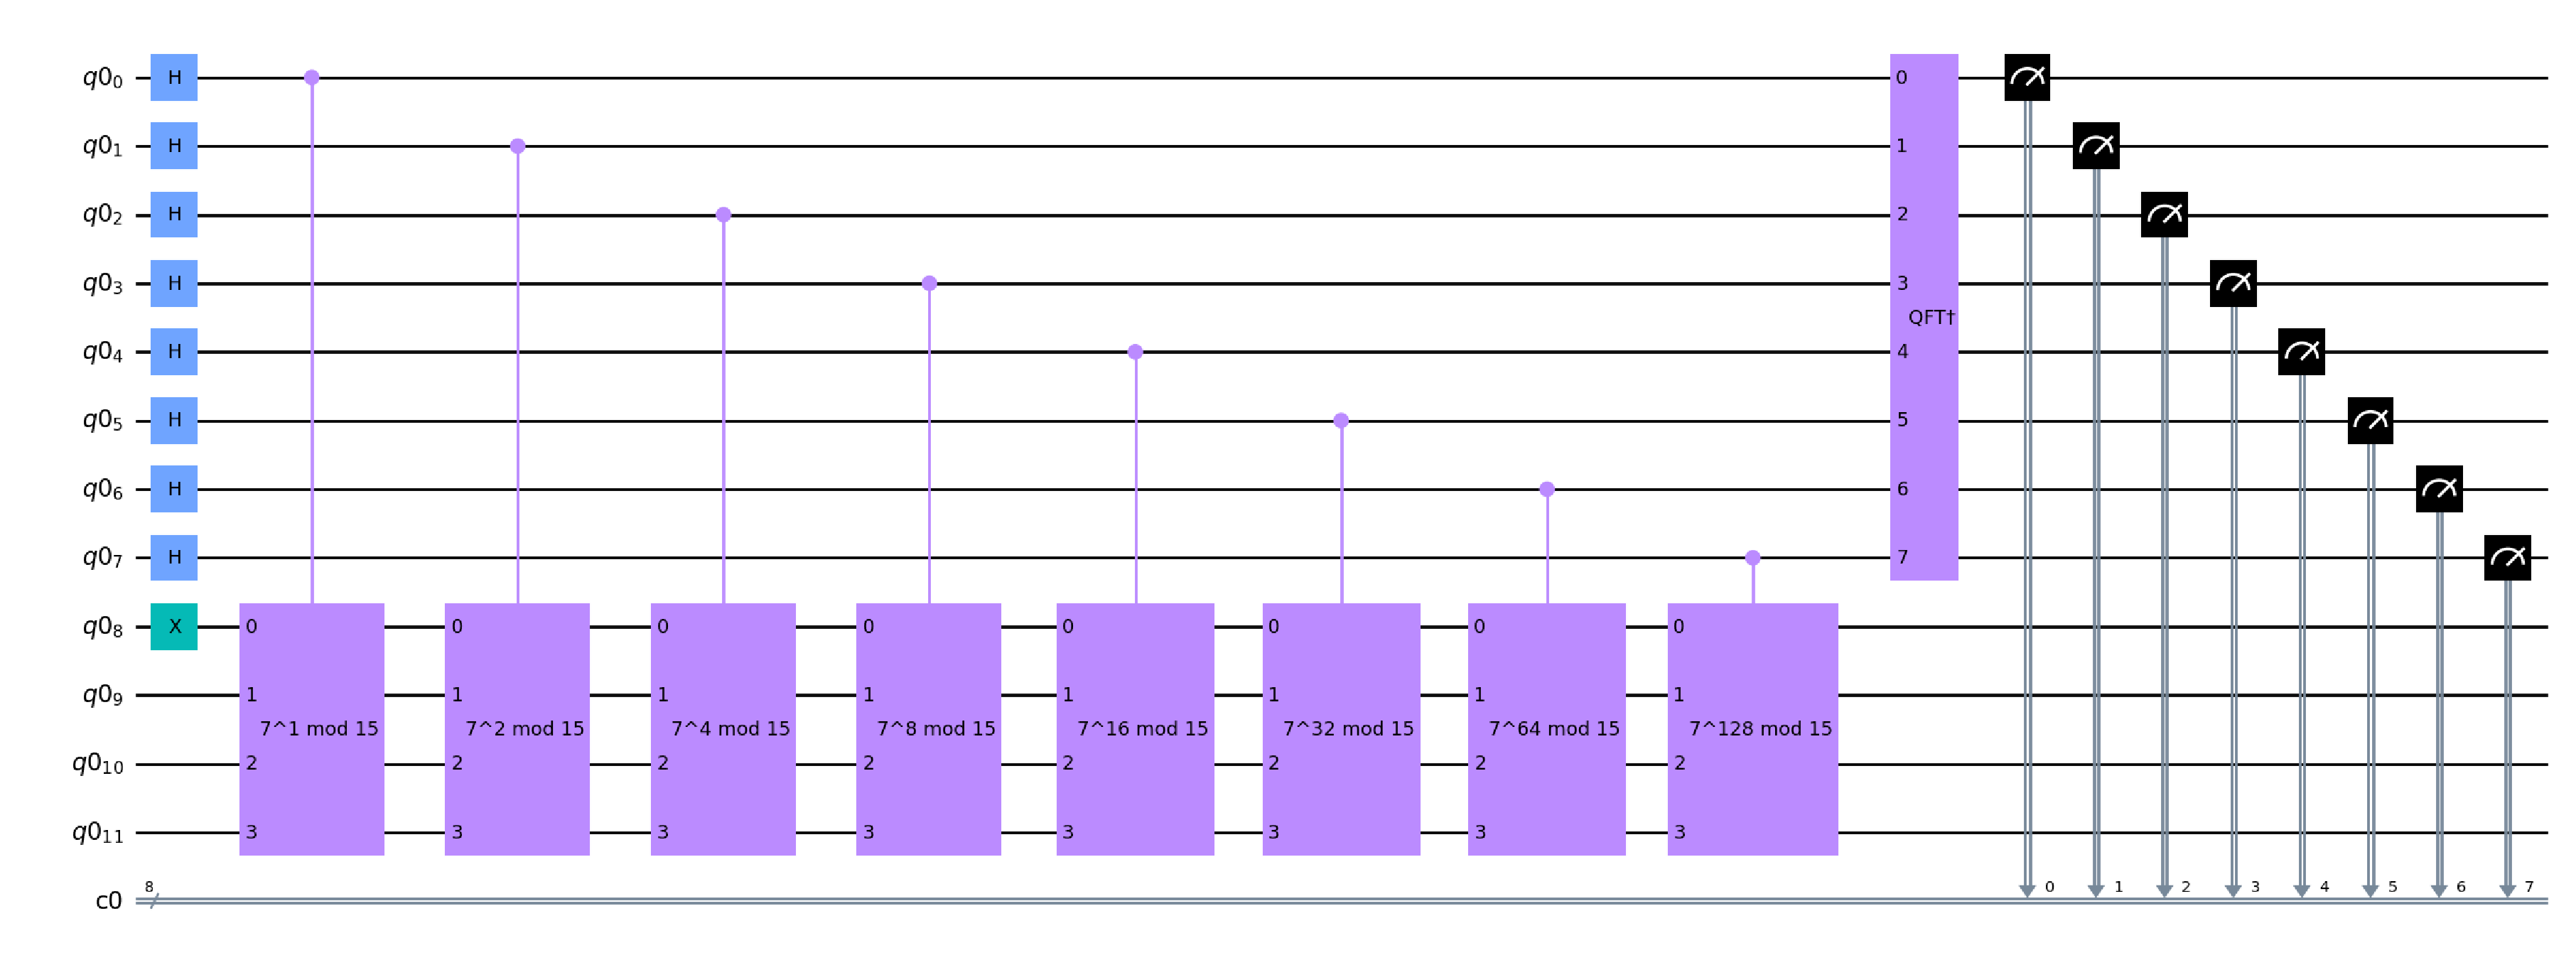
\includegraphics[width=0.8\textwidth]{images/appendix/out5.eps}\end{center}
\end{pyout}

Afin d'étudier son fonctionnement théorique, nous allons simuler le circuit quantique.
Pour cela, on utilise le simulateur que l'on définit, puis le circuit est transpilé, donc modifié afin
de correspondre aux portes quantiques disponibles sur le simulateur.
Le circuit est ensuite exécuté sur le simulateur, et les résultats sont récupérés pour être affichés
sous forme d'histogramme.\\

\begin{pyin}
aer_sim = Aer.get_backend('aer_simulator')
t_qc = transpile(qc, aer_sim)
counts = aer_sim.run(t_qc).result().get_counts()
plot_histogram(counts)
\end{pyin}

\begin{pyout}
;@ \begin{center}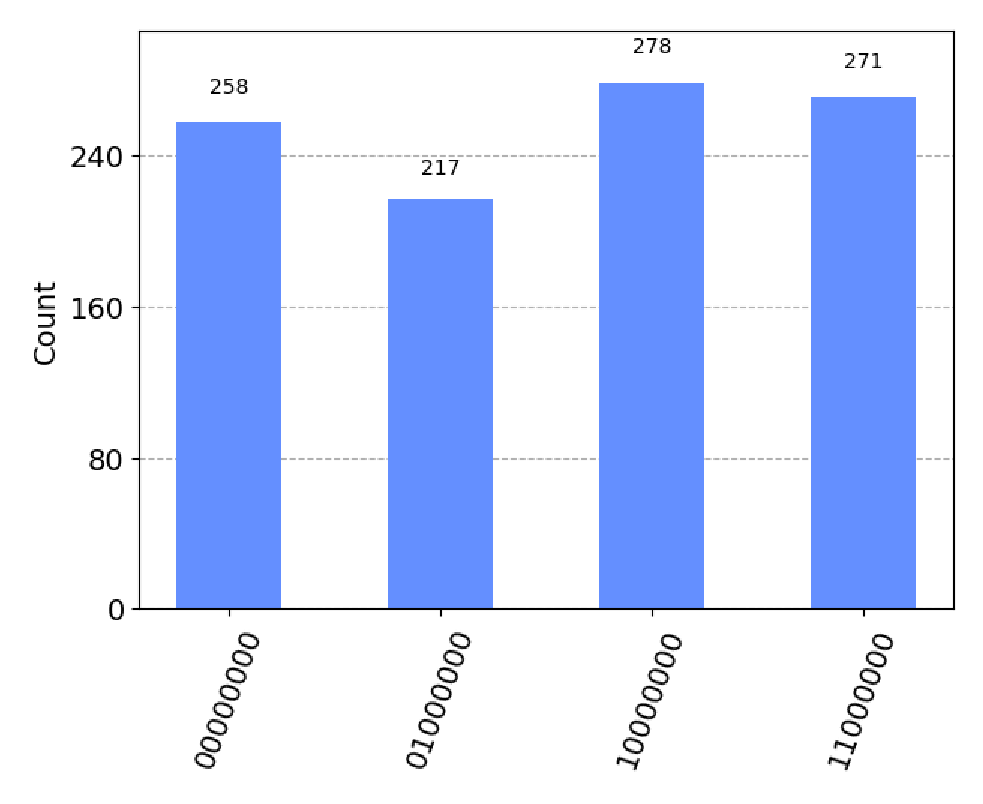
\includegraphics[width=0.8\textwidth]{images/appendix/out6.eps}\end{center}
\end{pyout}

Dans ce cas, les résultats doivent encore être traités afin de pouvoir être exploités.
Les cellules suivantes permettent d'effectuer toutes les opérations nécessaires pour
pouvoir les utiliser.\\

\begin{pyin}
rows, measured_phases = [], []
for output in counts:
    decimal = int(output, 2)  # Convert (base 2) string to decimal
    phase = decimal/(2**N_COUNT)  # Find corresponding eigenvalue
    measured_phases.append(phase)
    # Add these values to the rows in our table:
    rows.append([f"{output}(bin) = {decimal:>3}(dec)",
                 f"{decimal}/{2**N_COUNT} = {phase:.2f}"])
# Print the rows in a table
headers=["Register Output", "Phase"]
df = pd.DataFrame(rows, columns=headers)
print(df)
\end{pyin}

\begin{pyprint}
            Register Output           Phase
0  10000000(bin) = 128(dec)  128/256 = 0.50
1  00000000(bin) =   0(dec)    0/256 = 0.00
2  11000000(bin) = 192(dec)  192/256 = 0.75
3  01000000(bin) =  64(dec)   64/256 = 0.25
\end{pyprint}

\begin{pyin}
rows = []
for phase in measured_phases:
    frac = Fraction(phase).limit_denominator(15)
    rows.append([phase,
                 f"{frac.numerator}/{frac.denominator}",
                 frac.denominator])
# Print as a table
headers=["Phase", "Fraction", "Guess for r"]
df = pd.DataFrame(rows, columns=headers)
print(df)
\end{pyin}

\begin{pyprint}
   Phase Fraction  Guess for r
0   0.50      1/2            2
1   0.00      0/1            1
2   0.75      3/4            4
3   0.25      1/4            4
\end{pyprint}

Afin d'avoir une idée à quoi cela ressemblerait un tel circuit sur un ordinateur quantique réel,
nous pouvons le simuler en utilisant des bruits qui sont calqués sur ceux des ordinateurs quantiques
réels.\\

\begin{pyin}
from qiskit import QuantumCircuit, QuantumRegister, Aer, execute
from qiskit.providers.fake_provider import FakeMelbourne
backend = FakeMelbourne()
shots=1024
\end{pyin}

Dans cette étape, des opérations d'affichage des étapes du programme sont effectuées afin de pouvoir
suivre l'avancement de celui-ci, car cela peut prendre un certain temps.
Notons que dans ce cas, on voit que le circuit est inexploitable, parce que les résultats sont trop bruités
et le graphe est illisible.\\

\begin{pyin}
print('Start...')
qc_trans = transpile(qc, backend, optimization_level=1)
print('Done... (1/?)')
results = execute(qc_trans, backend, shots=shots).result()
print('Done... (2/?)')
counts_re = results.get_counts()
plot_histogram(counts_re)
\end{pyin}

\begin{pyprint}
Start...
Done... (1/?)
Done... (2/?)
\end{pyprint}

\begin{pyout}
;@ \begin{center}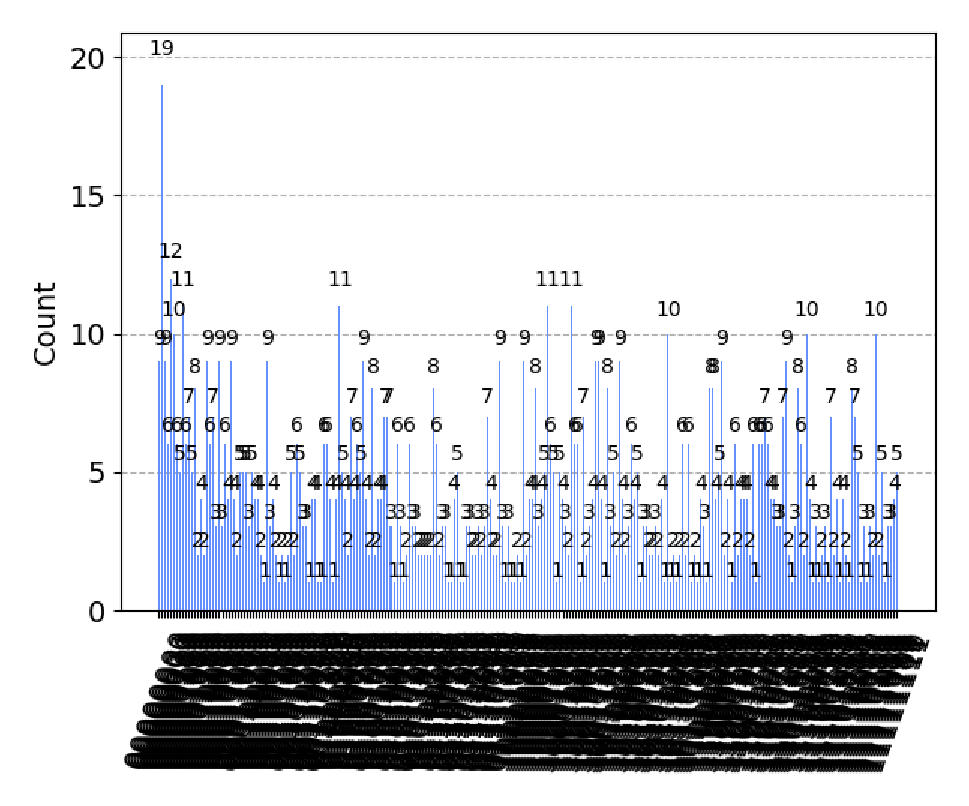
\includegraphics[width=0.8\textwidth]{images/appendix/out10.eps}\end{center}
\end{pyout}

On peut ensuite essayer de corriger les erreurs en utilisant la méthode de correction de mesure
proposée par \emph{Qiskit}.
On voit que cela fait ressortir certains résultats, mais que le graphe reste assez bruité.\\

\begin{pyin}
from qiskit.utils.mitigation import complete_meas_cal, CompleteMeasFitter
meas_calibs, state_labels = complete_meas_cal(qubit_list=[0,1,2,3,4,5,6,7], circlabel='mcal')
\end{pyin}

\begin{pyin}
job = execute(meas_calibs, backend=backend, shots=shots)
cal_results = job.result()

meas_fitter = CompleteMeasFitter(cal_results, state_labels, circlabel='mcal')
\end{pyin}

\begin{pyin}
meas_filter = meas_fitter.filter

mitigated_results = meas_filter.apply(results)
mitigated_counts = mitigated_results.get_counts(0)
\end{pyin}

\begin{pyin}
plot_histogram([counts_re, mitigated_counts], legend=['noisy', 'mitigated'])
\end{pyin}

\begin{pyout}
;@ \begin{center}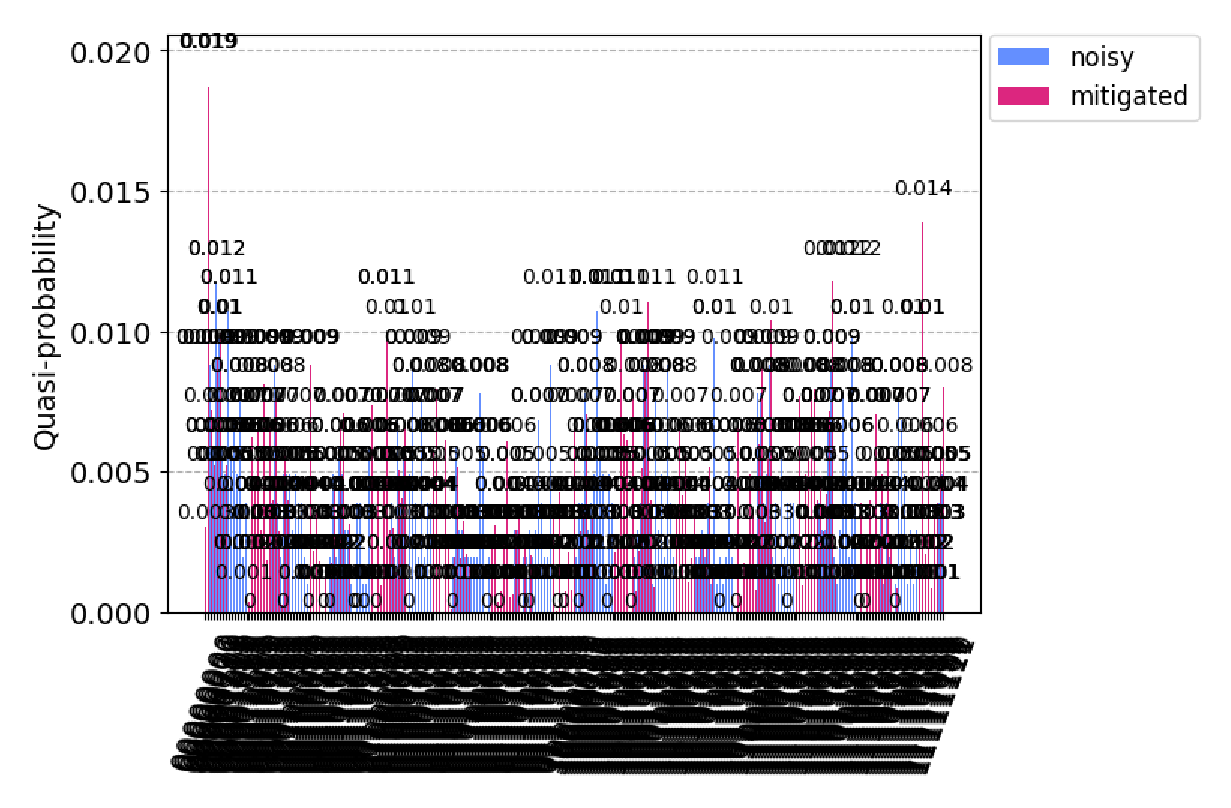
\includegraphics[width=0.8\textwidth]{images/appendix/out14.eps}\end{center}
\end{pyout}

Finalement, le clou du spectacle, nous allons envoyer le circuit sur un ordinateur quantique réel.
Dans ce cas, nous utilisons le service \emph{IBMQ}, qui permet d'envoyer des circuits sur les ordinateurs
quantiques d'IBM\@.
Afin de garder le token secret, la fonction d'utilisation d'un compte enregistré est utilisée.\\

\begin{pyin}
from qiskit import IBMQ
from qiskit.providers.ibmq import least_busy
from qiskit.tools import job_monitor
from qiskit_ibm_runtime import QiskitRuntimeService

shots = 8192
provider = IBMQ.load_account()

service = QiskitRuntimeService()
\end{pyin}

\begin{pyprint}
C:\Users\romai\AppData\Local\Temp\ipykernel_28196\2450165869.py:7: DeprecationWarning: The qiskit.IBMQ entrypoint and the qiskit-ibmq-provider package (accessible from 'qiskit.providers.ibmq') are deprecated and will be removed in a future release. Instead you should use the qiskit-ibm-provider package which is accessible from 'qiskit_ibm_provider'. You can install it with 'pip install qiskit_ibm_provider'. Just replace 'qiskit.IBMQ' with 'qiskit_ibm_provider.IBMProvider'
  provider = IBMQ.load_account()
\end{pyprint}

Nous créons ensuite le circuit quantique, qui possède 7 qubits, le maximum disponible sur les ordinateurs
quantiques mis à disposition gratuitement par IBM\@.\\

\begin{pyin}
N_COUNT = 3  # number of counting qubits
a = 7
# Specify variables

# Create QuantumCircuit with N_COUNT counting qubits
# plus 4 qubits for U to act on
qr = QuantumRegister(N_COUNT + 4)
cr = ClassicalRegister(N_COUNT)
qc = QuantumCircuit(qr, cr)

# Initialize counting qubits
# in state |+>
for q in range(N_COUNT):
    qc.h(q)

# And auxiliary register in state |1>
qc.x(N_COUNT)

# Do controlled-U operations
for q in range(N_COUNT):
    qc.append(c_amod15(a, 2**q),
              [q] + [i+N_COUNT for i in range(4)])

# Do inverse-QFT
qc.append(qft_dagger(N_COUNT), range(N_COUNT))

# Measure circuit
qc.measure(range(N_COUNT), range(N_COUNT))

# qc.draw(output='mpl')
\end{pyin}

Sont commentés les lignes permettant de choisir un ordinateur quantique réel sur lequel envoyer le circuit,
en choisissant celui qui est le moins occupé et qui répond à certains critères.
Néanmoins, dans ce cas, nous allons envoyer utiliser les résultats d'un circuit envoyé précédemment.\\

\begin{pyin}
from qiskit.utils.mitigation import complete_meas_cal, CompleteMeasFitter
meas_calibs, state_labels = complete_meas_cal(qubit_list=[0,1,2], circlabel='mcal')

# device = least_busy(
#     provider.backends(
#         filters=lambda x: x.configuration().n_qubits >= 7
#                           and not x.configuration().simulator                # Not a simulator
#                           and x.status().operational == True                 # Operational backend
#     )
# )
#
# display(device)
#
# Submit a job.
# jobcal = execute(meas_calibs, backend=device)
# job_monitor(jobcal)
# job = execute(qc, backend=device, optimization_level=3, shots=shots)
# job_monitor(job)

# Execute the 31.08.2023 on ibm_nairobi
jobcal = service.job('cjo1ngpdll3gjfa1lne0')
job = service.job('cjo1svhpthn588jkkphg')

count = job.result().get_counts()
meas_cal = jobcal.result()

meas_fitter = CompleteMeasFitter(meas_cal, state_labels, circlabel='mcal')
meas_filter = meas_fitter.filter

mitigated_results = meas_filter.apply(job.result())
mitigated_counts = mitigated_results.get_counts()

plot_histogram([count, mitigated_counts], legend=['noisy', 'mitigated'])
\end{pyin}

\begin{pyout}
;@ \begin{center}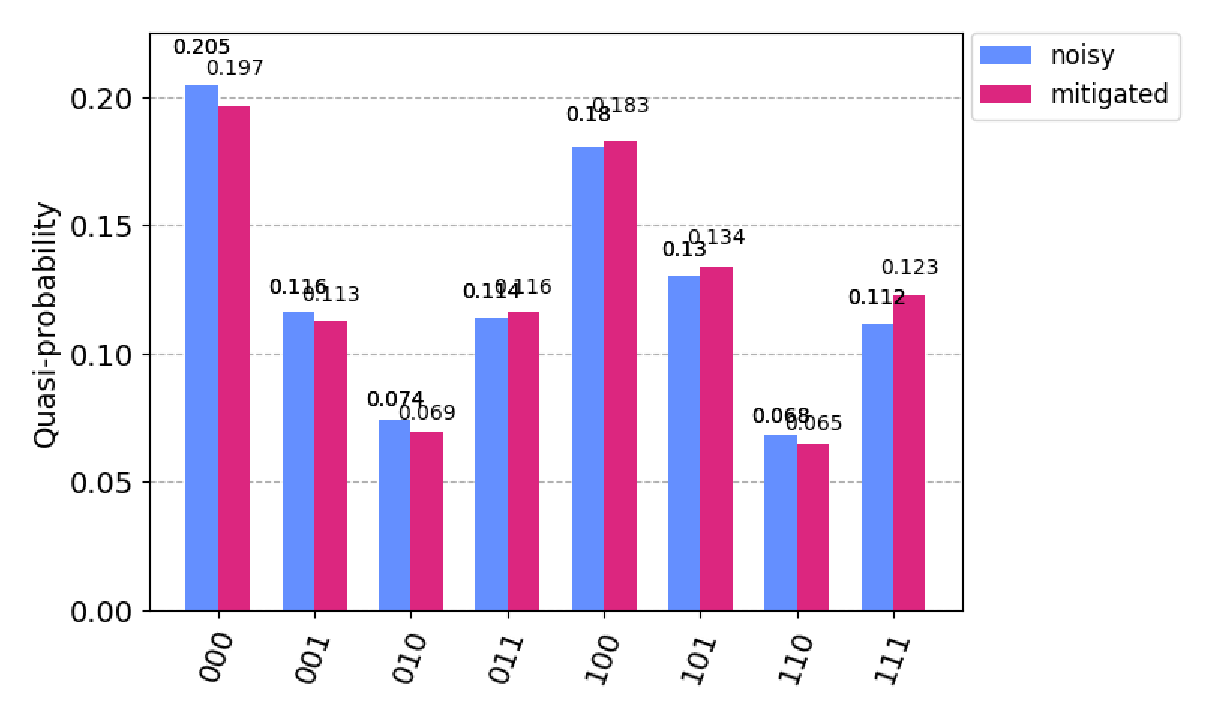
\includegraphics[width=0.7\textwidth]{images/appendix/out16.eps}\end{center}
\end{pyout}

Nous voyons donc d'où viennent les résultats obtenus dans le chapitre~\ref{ch:algorithme-de-shor}.
Par cet exemple, cela offre aussi un aperçu de la manière dont les circuits quantiques sont construits
et utilisés dans ce document.
